\documentclass[../AP_Statistics.tex]{subfiles}

\begin{document}
	\section{Data Analysis}
		Statistics is the science of collecting and analyzing data. \\
		A data set is a collection of data on several \textbf{individuals}. These individuals can be anything. \\
		Data provides values for \textbf{variables}, which describe some characteristic of an individual. \\
		\textbf{Categorical variables} assign labels that place each individual into one of several groups, while \textbf{quantitative variables} provide values that describe or measure some characteristic. \\
		Quantitative variables can either be \textbf{discrete}, having some countable set of possible values, or \textbf{continuous} having an uncountably infinite set of possible values. \\
		A variable's \textbf{distribution} describes the frequency with which a variable takes on its possible values.
		\subsection{Analyzing Categorical Data}
			A \textbf{frequency table} shows the number of individuals that have a certain value while a \textbf{relative frequency table} shows the percentage of all individuals in the data set that have that particular value. \\
			\textbf{Bar graphs} show each category as a bar, the height of which corresponds to its frequency. \\
			\begin{center}
				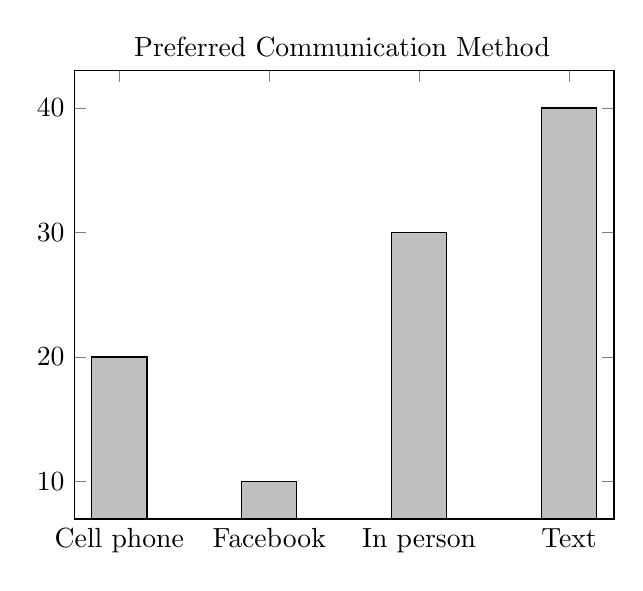
\begin{tikzpicture}
					\begin{axis}[bar width = 20pt, symbolic x coords = {Cell phone, Facebook, In person, Text}, xtick = data]
						\addplot[ybar, fill = lightgray] coordinates{(Cell phone, 20) (Facebook, 10) (In person, 30) (Text, 40)};
					\end{axis}
					\node at (3.4,6) {Preferred Communication Method};
				\end{tikzpicture}
			\end{center}
			\textbf{Pie charts} show each category as some fraction of a circle that is bounded by two radii. The areas of each slice is proportional to the frequency.
	\section{Modeling Distributions of Data}
		\subsection{Describing Location in a Distribution}
		
\end{document}